\documentclass[conference]{IEEEtran}
\IEEEoverridecommandlockouts
% The preceding line is only needed to identify funding in the first footnote. If that is unneeded, please comment it out.
\usepackage{cite}
\usepackage{amsmath,amssymb,amsfonts}
\usepackage{algorithmic}
\usepackage{graphicx}
\usepackage{textcomp}
\usepackage{booktabs}
\usepackage{xcolor}
\def\BibTeX{{\rm B\kern-.05em{\sc i\kern-.025em b}\kern-.08em
    T\kern-.1667em\lower.7ex\hbox{E}\kern-.125emX}}
\usepackage{subfig}
\usepackage{xspace}
\newcommand{\system}{\textit{BriskSeed}\xspace}
\begin{document}

\title{BriskSeed: Online History-Guided Reuse for Accelerating Dynamic Approximate Nearest Neighbor Search}

\author{\IEEEauthorblockN{Hongru Gao, Shuhao Zhang*, Xiaofei Liao, Hai Jin}
\IEEEauthorblockA{National Engineering Research Center for Big Data Technology and System,\\
 Services Computing Technology and System Lab, Cluster and Grid Computing Lab,\\School of Computer Science and Technology,  Huazhong University of Science and Technology,
Wuhan, China \\
\{hrgao, shuhao\_zhang, xfliao, hjin\}@hust.edu.cn}

}

\maketitle
\begin{abstract}
Approximate Nearest Neighbor Search (ANNS) is a core primitive in modern data systems, 
but most high-performance graph-based indices are optimized for static workloads 
rather than continuously evolving data. Under streaming insertions and deletions, 
pre-computed search guidance quickly becomes stale, causing either lower query efficiency 
or expensive re-optimization. To address this challenge, we present BriskSeed, 
a pluggable optimization module for dynamic ANNS.
Its key idea is to turn past successful search outcomes into reusable search primitives, referred to as \textit{seeds}, while controlling the overhead and risk of stale reuse under evolving data.
Specifically, BriskSeed integrates seed storage, seed-guided search, and reliability control into a unified online workflow: it organizes seeds in a two-tier utility-aware 
storage scheme, activates them through exact lookup and bounded semantic probing, and validates them through 
a lightweight acceptance-and-fallback policy.
This design preserves a compact set of high-value seeds under distribution drift while remaining compatible with existing ANNS backends.
We evaluate BriskSeed on
\textbf{CANDOR-Bench}, a streaming ANNS benchmark framework, across multiple ANNS backends under a unified plugin interface.
Experimental results show that BriskSeed 
consistently improves end-to-end search efficiency while sustaining 
competitive recall under high update rates.
\end{abstract}

\begin{IEEEkeywords}
Approximate Nearest Neighbor Search, Data Structure, Graph Index.
\end{IEEEkeywords}

\section{Introduction}
Approximate Nearest Neighbor Search (ANNS) is a core primitive in modern data systems, including Retrieval-Augmented Generation (RAG), recommendation, and anomaly detection~\cite{Zhong20255017}. Graph-based indices such as HNSW~\cite{Jayaram2019, Malkov2020824} are widely adopted because they offer strong recall-latency trade-offs at scale. Their search process relies on graph traversal over non-contiguous memory regions, where random access and cache misses often dominate runtime. Existing acceleration techniques generally follow two directions: system-level optimizations that compute faster (e.g., layout, SIMD, quantization)~\cite{Gou2025, Wang2025, Zhong20255017}, and algorithm-level optimizations that compute less (e.g., pruning and distance estimation)~\cite{Chen20233225, Gao2023, Song2025}.

Despite substantial progress, most optimizations are developed for static or slowly evolving data snapshots. In practical streaming systems, vectors are continuously inserted and deleted, creating a temporal mismatch: auxiliary search metadata that is effective at time $t$ may become stale at time $t+\Delta$. This mismatch is particularly pronounced in high-rate pipelines (e.g., social-content ingestion), where distribution shift and index-topology evolution occur concurrently.

This setting induces a fundamental efficiency-maintenance dilemma, illustrated in Figure~\ref{fig:motivation}. Without maintenance, query throughput (QPS) degrades as optimization hints lose validity (Figure~\ref{fig:stale-hint}); with frequent global re-optimization, maintenance overhead dominates end-to-end cost (Figure~\ref{fig:reopt-cost}). Consequently, the key challenge is not merely how to accelerate search, but how to keep acceleration \emph{continuously valid} under ongoing updates.

\begin{figure}
	\centering
	\subfloat[Staleness-induced performance decay]{
		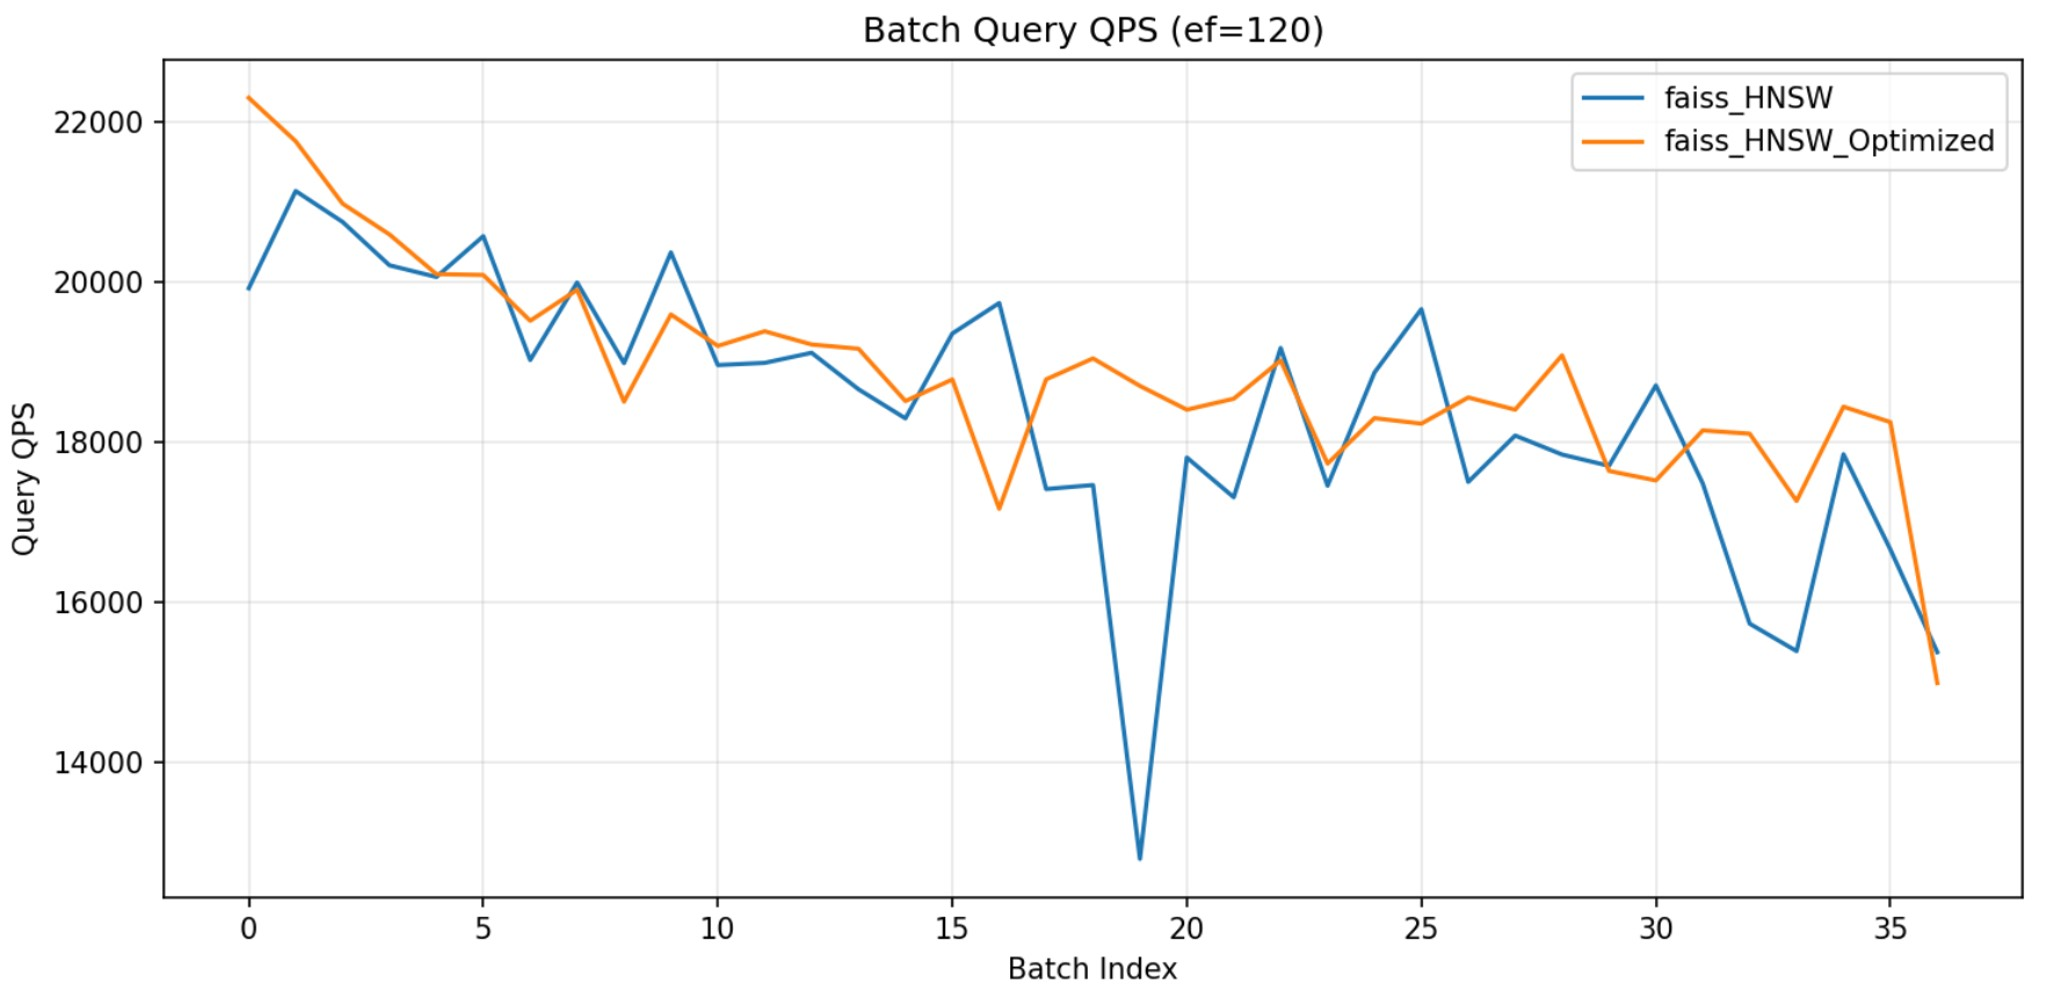
\includegraphics[width=\columnwidth]{figures/figure1a.jpg}
		\label{fig:stale-hint}
	}
    \\
    \subfloat[Cost of frequent global re-optimization]{
		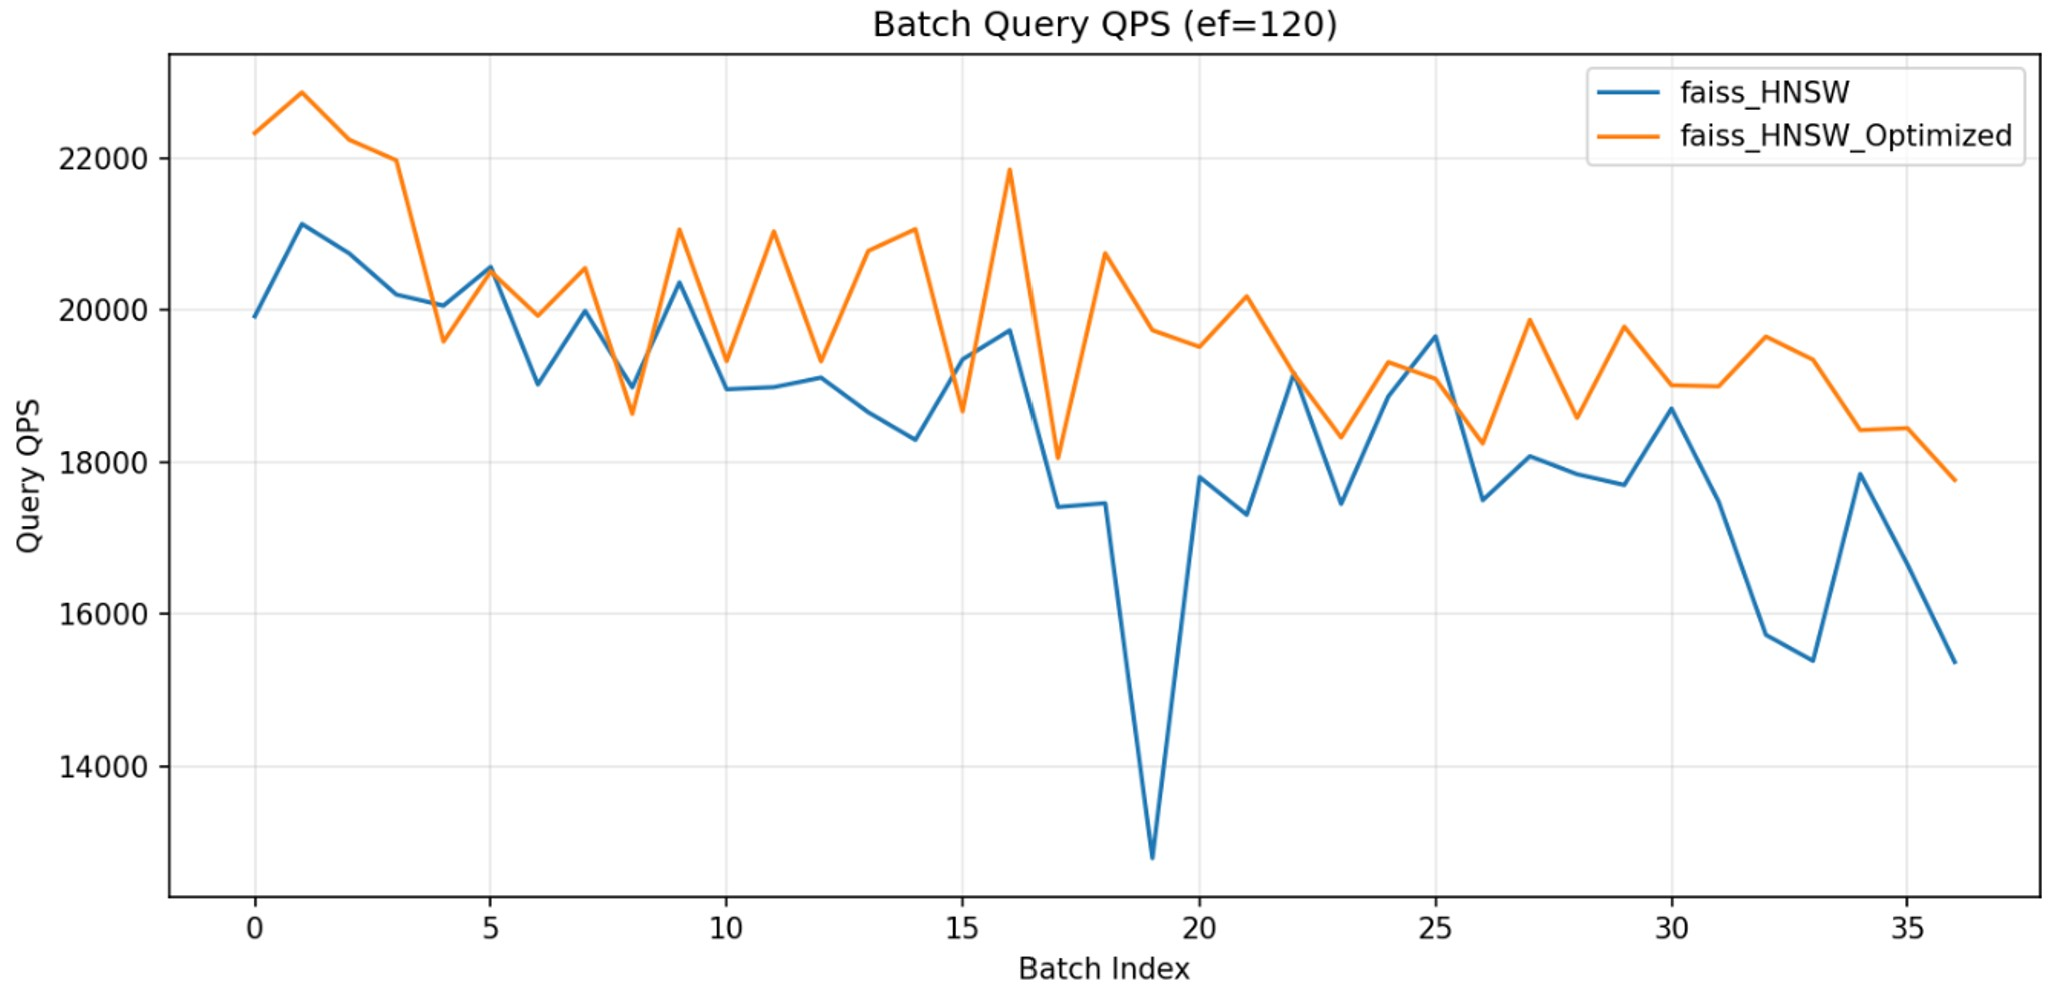
\includegraphics[width=\columnwidth]{figures/figure1b.jpg}
		\label{fig:reopt-cost}
	}
    \caption{Motivating trade-off in dynamic ANNS: stale hints hurt search efficiency, while aggressive global maintenance hurts amortized throughput.}
	\label{fig:motivation}
\end{figure}

\noindent\textbf{Key idea and design overview.}
Rather than optimizing static snapshots, StreamSeed formulates acceleration as an online control problem under drift.
The design is organized around two aspects.
\textbf{Design Aspect I (Workload-aligned reuse under drift)} renders hint reuse selective and self-correcting: reuse is enabled when recent evidence indicates positive utility and disabled when confidence degrades.
\textbf{Design Aspect II (Backend-decoupled control interface)} separates policy logic from backend mechanics, enabling a shared policy family to be reused across dynamic ANN backends with low integration overhead.

\noindent\textbf{Contributions.}
This paper makes the following contributions:
\begin{itemize}
	\item We formalize the stale-hint problem in streaming ANNS as an amortized search-maintenance optimization problem, clarifying why static accelerations degrade in dynamic regimes.
	\item We present StreamSeed with two explicit design aspects: workload-aligned reuse under drift and a backend-decoupled control interface.
	\item We implement StreamSeed in CANDOR-Bench through a pluginized policy--adapter--runtime structure and runbook-driven configuration, enabling reproducible dynamic evaluations across workloads.
	\item We provide empirical results and ablations showing that unified query-hint control improves end-to-end efficiency while maintaining competitive recall under high update rates.
\end{itemize}

\noindent\textbf{Paper organization.}
Section 2 formalizes the problem and preliminaries.
Section 3 presents the StreamSeed design.
Section 4 describes implementation details in CANDOR-Bench.
Section 5 reports evaluation and ablation results.
Section 6 discusses related work, and Section 7 concludes.

\section{Problem Formulation and Motivation}
This section first formulates the problem statement in Section~2.1. Section~2.2 then presents two key observations that motivate our design,
 namely temporal locality across updates and skew in practical query workloads. Finally, Section~2.3 discusses the main challenges in designing BriskSeed.

\subsection{Problem Statement}

We begin with the standard Approximate Nearest Neighbor Search(ANNS) definition and then extend it to the dynamic setting considered in this paper.

\begin{table}[thb]
  \caption{Summary of terminologies}
  \label{tab:symbols}
  \begin{tabular}{lp{6.3cm}}
    \toprule
    Symbol & Description\\
    \midrule
    $\mathcal{D}$ & Vector dataset. \\
    $\mathcal{D}_r$ & Vector dataset state after applying the batch updates at round $r$. \\
    $\widehat{N}_k(q)$ & Approximate top-$k$ result set of query $q$. \\
    $N_k^{\ast}(q)$ & Exact top-$k$ nearest-neighbor set of query $q$. \\
    $\mathrm{Recall@}k(q)$ & Recall of the approximate top-$k$ result for query $q$. \\
    $\mathcal{U}_r$ & Batch updates at round $r$. \\
    $\mathcal{Q}_r$ & Batch queries executed at round $r$. \\
	$\mathcal{R}$ & The number of rounds we evaluate. \\
    $L_{\mathrm{search}}(q)$ & Search latency of query $q$. \\
    $L_{\mathrm{maintain}}(\mathcal{U}_r)$ & Maintenance cost triggered by batch updates $\mathcal{U}_r$. \\
    $\mathrm{QPS}(R)$ & Average query throughput within $\mathrm{R}$ rounds. \\
    $\tau$ & Tolerance threshold for Recall@$k$. \\
    \bottomrule
  \end{tabular}
\end{table}

\noindent\textbf{Definition 1 (ANNS).}
Given a vector dataset $\mathcal{D}\subset\mathbb{R}^d$, a query $q\in\mathbb{R}^d$, and an integer $k$, ANNS returns an approximate top-$k$ set $\widehat{N}_k(q)$ that approximates the exact nearest-neighbor set $N_k^{\ast}(q)$ under a distance metric. The standard search quality metric is Recall@$k$:
\begin{equation}
\mathrm{Recall@}k(q)=\frac{|\widehat{N}_k(q)\cap N_k^{\ast}(q)|}{k}.
\end{equation}

Definition 1 captures the static ANNS setting, where the vector dataset and index structure remain fixed during queries. 
In practical systems, however, vectors are continuously inserted and deleted, and therefore the ANNS index also evolves over time. 
To model this setting, we extend ANNS to a dynamic formulation and adopt the serialized round-based execution model used in CANDOR-Bench.

\noindent\textbf{Definition 2 (Dynamic ANNS).}
Dynamic ANNS operates on a time-evolving dataset in rounds. At each round $r$, the system first applies a batch updates $\mathcal{U}_r$ (insertions/deletions) 
to transform $\mathcal{D}_{r-1}$ into $\mathcal{D}_r$, and then executes a batch queries $\mathcal{Q}_r$ on $\mathcal{D}_r$. The index structure is updated online across rounds.

In this setting, many optimizations developed for static ANNS become less effective as updates accumulate, including layout restructuring, quantization-based acceleration, 
and globally precomputed auxiliary guidance. As their effectiveness decays, query throughput drops and recall may also deteriorate. Frequent re-optimization is not a viable
solution either, because its maintenance overhead can dominate end-to-end cost, as shown in Figure~\ref{fig:reopt-cost}. This dilemma motivates the following problem.

\noindent\textbf{Problem Statement.}
The goal is to maximize end-to-end query throughput in dynamic ANNS under continuous updates, while preserving comparable recall to baselines. In dynamic ANNS, low query latency is meaningful 
only if the maintenance required to sustain it is also affordable. We therefore account for both search cost and maintenance cost in the end-to-end throughput objective across update-query rounds.

Let $\mathcal{Q}_r$ denote the query batch at round $r$, and let $n_r = |\mathcal{Q}_r|$ be the number of queries in that round. Over an evaluation horizon of $R$ rounds, we define the total search cost and total maintenance cost as
\begin{equation}
L_s(R)=\sum_{r=1}^{R}\sum_{q\in\mathcal{Q}_r} L_{\mathrm{search}}(q), \quad L_m(R)=\sum_{r=1}^{R} L_{\mathrm{maintain}}(\mathcal{U}_r).
\end{equation}
The corresponding query throughput is
\begin{equation}
\mathrm{QPS}(R)=\frac{\sum_{r=1}^{R} n_r}{L_s(R)+L_m(R)}.
\end{equation}

Our objective is to maximize $\mathrm{QPS}(R)$ subject to an average recall constraint:
\begin{equation}
\begin{aligned}
\max \quad & \mathrm{QPS}(R) \\
\text{s.t.}\quad &
\frac{1}{\sum_{r=1}^{R} n_r}
\sum_{r=1}^{R}\sum_{q\in\mathcal{Q}_r}\mathrm{Recall@}k(q)
\ge
\tau \cdot \overline{\mathrm{Recall}}^{\mathrm{baseline}},
\end{aligned}
\end{equation}
where
\begin{equation}
\overline{\mathrm{Recall}}^{\mathrm{baseline}}=
\frac{1}{\sum_{r=1}^{R} n_r}
\sum_{r=1}^{R}\sum_{q\in\mathcal{Q}_r}\mathrm{Recall@}k(q)^{\mathrm{baseline}},
\end{equation}
and $\tau \in (0,1]$ controls the required recall ratio relative to the baseline.


\begin{figure}
	\centering
	\subfloat[Overlapped top-$k$ results across updates]{
		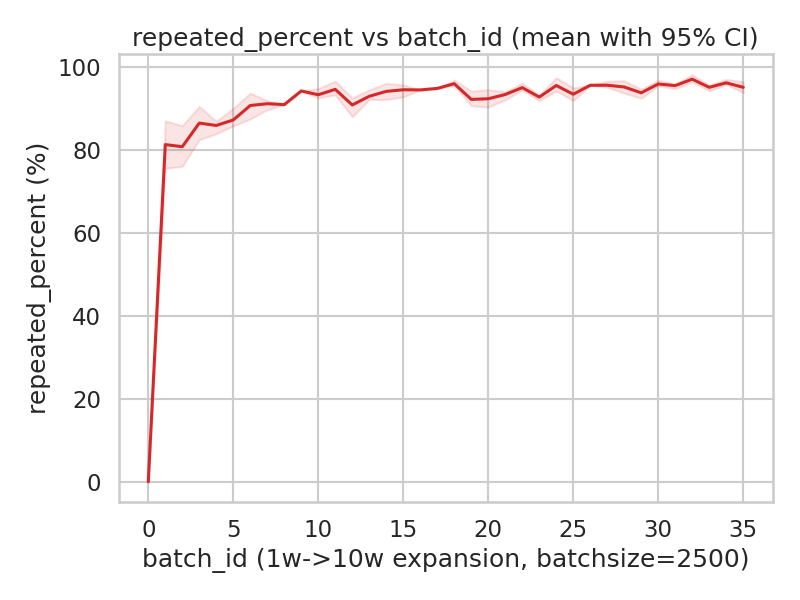
\includegraphics[width=0.48\columnwidth]{figures/figure2a.png}
		\label{fig:repeat results}
	}
    \subfloat[Skewness in query hotspot distribution]{
		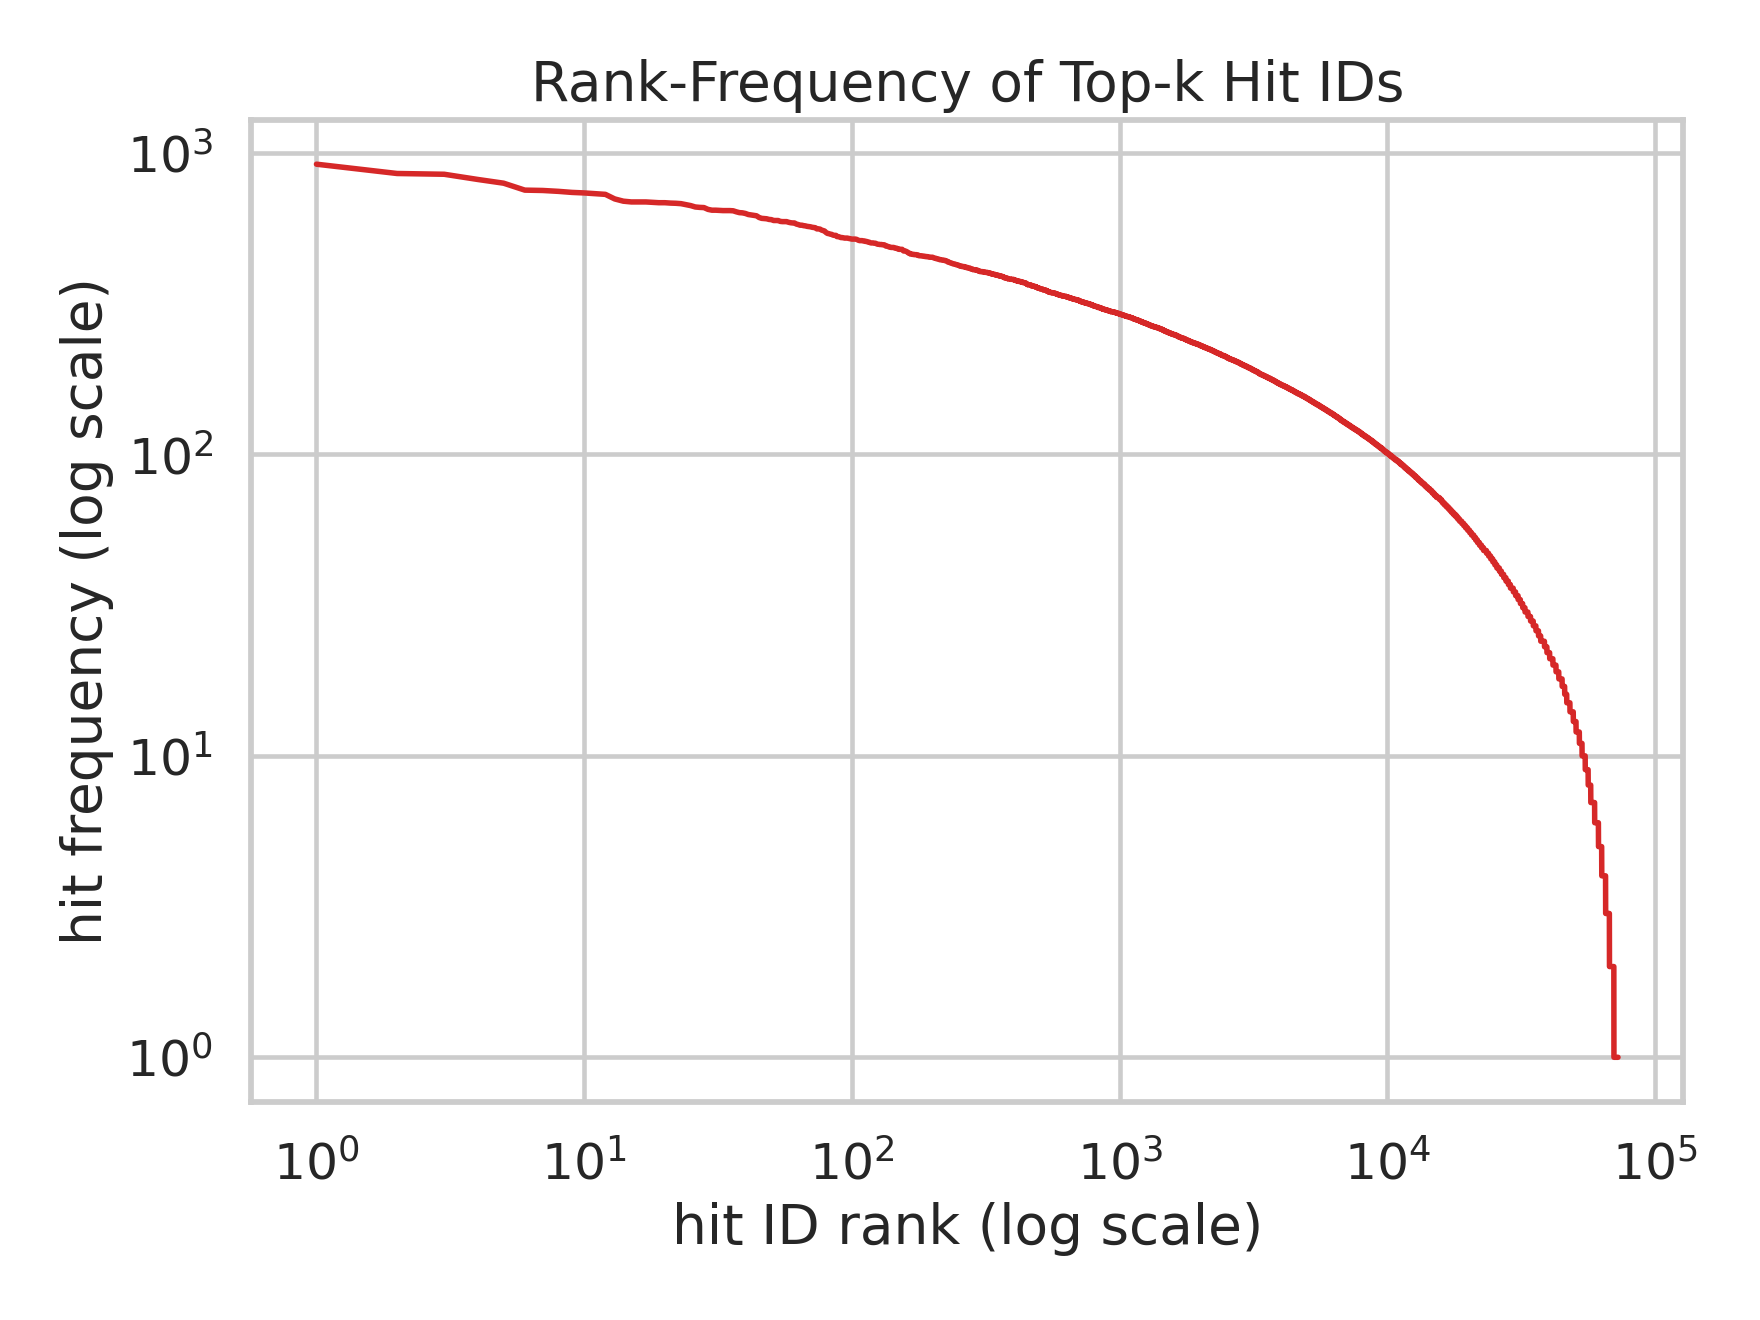
\includegraphics[width=0.48\columnwidth]{figures/figure2b.png}
		\label{fig:skewness}
	}
    \caption{Key observations in dynamic ANNS.}
	\label{fig:observation}
\end{figure}

\subsection{Key Observations}

To better understand the behavior of dynamic ANNS workloads, we conduct a preliminary empirical study and identify two key observations.

\noindent\textbf{Observation 1: Temporal locality across updates.} For the same query batch, the top-$k$ results often remain highly overlapping across nearby update rounds. 
As shown in Figure~\ref{fig:repeat results}, the 
overlap ratio of top-$k$ results quickly exceeds 80\% after the first few batches and remains around 95\% thereafter. This pattern indicates a form of 
\emph{temporal locality across updates}: although accumulated updates may gradually reduce the effectiveness of search acceleration, they do not immediately cause large 
changes in the query results. Therefore, recent high-quality search outcomes can potentially be reused for subsequent queries, as long as their 
reuse is bounded and adaptive.

\noindent\textbf{Observation 2: Long-tail skew in query-hit frequency.}
Across batch queries, the top-$k$ hit IDs often exhibit strong concentration rather than uniform coverage. As shown in Figure~\ref{fig:skewness}, the frequency 
of hit IDs follows a clear long-tail distribution: a small fraction of IDs is found very frequently, while the majority is rarely observed. This skew indicates 
that query-hit patterns in dynamic ANNS are highly uneven, and that not all recurring search outcomes are equally valuable for reuse. As a result, treating 
historical outcomes discriminately is likely to be cost-effective.


Taken together, these observations reveal both an opportunity and a principle for dynamic acceleration. Temporal locality suggests that recent search outcomes can be reused across updates, while long-tail skew suggests that such reuse should be selective rather than uniform. Therefore, an effective dynamic ANNS system should support both online reuse and cost-aware prioritization.


\subsection{Design Challenges}

Although the observations above reveal clear opportunities for dynamic ANNS acceleration, exploiting them efficiently and robustly under continuous updates remains non-trivial,
with the following challenges:

\noindent\textbf{Challenge 1: How should historical search outcomes be represented and stored?}
Although Observation 1 suggests that recent top-$k$ results can remain useful across nearby update rounds, high overlap does not imply that past outcomes can be reused unchanged. 
Instead, they should be retained as lightweight guidance for future search.
Therefore, the system must decide what information should be preserved from previous queries, how to represent it compactly, and how to store it under bounded memory overhead. 
Moreover, it must also balance retention and eviction so that useful outcomes remain available while stale ones are removed over time.

\noindent\textbf{Challenge 2: How can historical outcomes guide the search process?}
Even when historical outcomes are stored, turning them into effective search guidance remains non-trivial. 
The system must activate relevant outcomes for queries that do not exactly match previous ones, and use them to recover strong candidates without causing excessive search expansion. 
Moreover, Observation 2 suggests that reuse should be selective rather than uniform: highly recurring outcomes and long-tail outcomes may need to be handled differently in order to achieve good performance under bounded cost.
But, how to design such a selective reuse mechanism that can adapt to changing query-hit patterns is an open question.

\noindent\textbf{Challenge 3: How can historical-outcome reuse improve end-to-end query efficiency while preserving recall?}
Even when historical outcomes are well represented and selectively prioritized for search, reuse does not automatically improve both overall performance and recall, because the identified historical outcomes may still not reliable for current search. 
The system must therefore decide whether the reused search path should be accepted or whether it should fall back to the native search path, while keeping this decision process sufficiently lightweight. 
Designing such an acceptance-and-fallback mechanism is critical to ensuring that historical-outcome reuse improves efficiency without degrading recall.

Motivated by these challenges, we next present our design BriskSeed and elaborate on how it address Challenges 1-3.
\section{BriskSeed Design}
\label{sec:briskseed-design}

This section presents the full BriskSeed design for dynamic ANNS under continuous updates.
Section 3.1 introduces the design overview.
Section 3.2 describes the overall pipeline of BriskSeed.
Section 3.3 gives complexity, robustness, and challenge-wise implications.

\subsection{Design Overview}


Motivated by the observations and challenges in Section~2, we design \textbf{BriskSeed} as a three-layer online framework for accelerating dynamic ANNS. 
BriskSeed is built on a simple principle: historical search outcomes, referred to as \emph{seeds}, should be reused only when they can be represented compactly, activated selectively, and trusted safely under continuous updates. 
To this end, BriskSeed combines three layers that map directly to the three challenges in Section~2: Seed Storage Layer, Seed-Guided Search Layer, and Reliability Control Layer, as shown in Figure~\ref{fig:briskseed-design-overview}.

\noindent\textbf{(1) Seed Storage Layer (addresses Challenge 1).}
This layer determines how historical outcomes are represented, retained, and refreshed under bounded memory. 
To exploit the high top-$k$ overlap across nearby rounds, BriskSeed organizes reusable history in a two-tier seed storage: a hot-exact tier for highly recurring outcomes and a semantic-shared tier for compact long-tail coverage. 
Each seed stores historical top-$k$ IDs together with lightweight metadata needed for retrieval and maintenance. 
In this way, past outcomes are encoded as reusable guidance rather than final answers, while retention and eviction remain explicitly budgeted.

\noindent\textbf{(2) Seed-Guided Search Layer (addresses Challenge 2).}
This layer determines how stored outcomes guide query-time search. 
For each query, BriskSeed first retrieves seeds through exact lookup or bounded semantic probing, and then converts the selected seed into provisional candidates through bounded expansion. 
The guidance strategy is tier-aware: hot-exact seeds use one-hop neighbor expansion by default, while semantic-shared seeds use guarded multi-hop expansion only when one-hop evidence
is insufficient.
This design enables efficient reuse under skewed workloads while preventing uncontrolled search overhead.

\noindent\textbf{(3) Reliability Control Layer (addresses Challenge 3).}
This layer ensures that reuse improves end-to-end efficiency without degrading recall. 
Recovered candidates are checked by a lightweight query-level acceptance policy, where acceptance requires both strong local candidate quality and consistency with the seed's historical neighborhood. 
If either signal is weak, BriskSeed immediately falls back to the native search path. 
This explicit reliability gate ensures that acceleration remains beneficial while bounding recall risk.

These three layers are co-designed rather than independent. 
The seed storage layer determines what is reusable, the seed-guided search layer determines how reuse enters search, and the reliability control layer determines when recovered candidates are trustworthy enough to be accepted. 
Together, they form a bounded online reuse framework that aligns directly with the three design challenges and remains robust under continuous updates.



\begin{figure}[t]
\centering
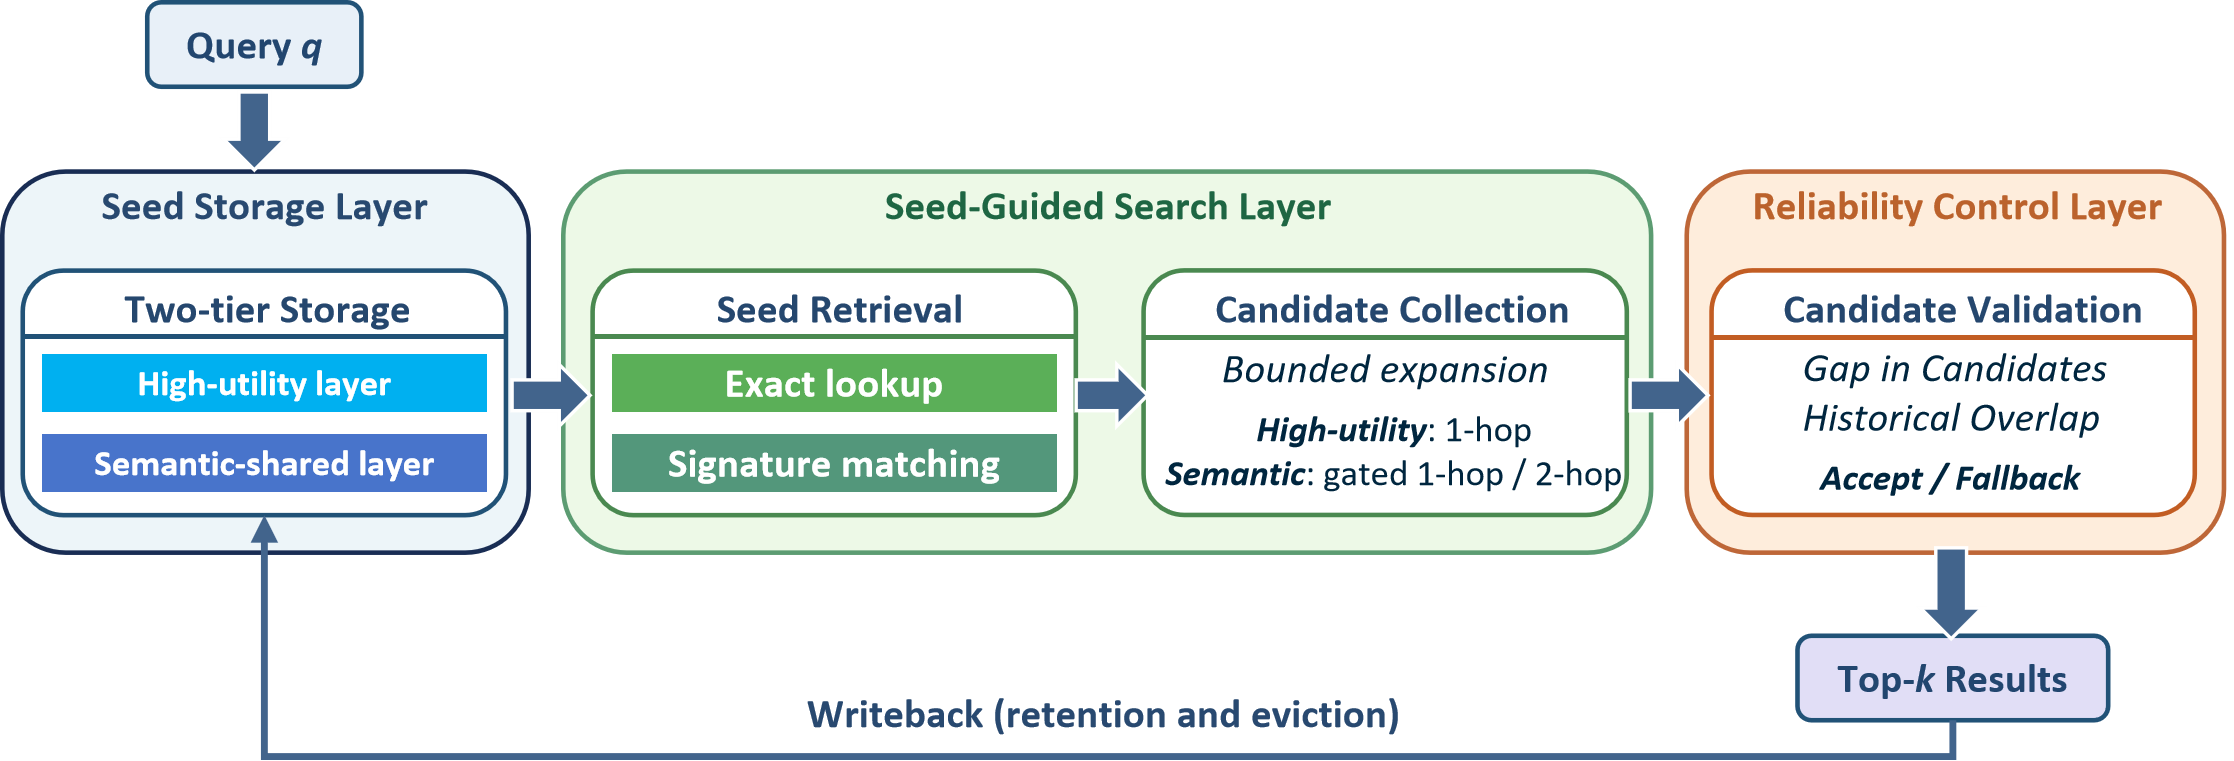
\includegraphics[width=\columnwidth]{figures/figure3.png}
\caption{BriskSeed design overview.}
\label{fig:briskseed-design-overview}
\end{figure}




\subsection{Unified Online Reuse Pipeline}
In this subsection, we detail the modules of BriskSeed and their interactions in the unified online reuse pipeline. Important symbols are summarized in Table~\ref{tab:pipeline-symbols}.

\subsubsection{Seed representation and storage}

\paragraph{Seed representation.}
We first define the representation of a seed, and then describe how such seeds are organized in the storage.

Each seed is stored as
\begin{equation}
r=\langle \mathbf{z}, n_b, \beta, \rho \rangle,
\end{equation}
where $\mathbf{z}\in\mathbb{N}^k$ is the historical top-$k$ result IDs used as reuse anchors, $n_b$ is the seed birth time (when the seed was created), $\beta$ identifies the source query ID (which query generated this seed), and $\rho$ records the successful reuse count. The anchor set $\mathbf{z}$ serves as the starting points for subsequent reuse, 
while the remaining metadata summarize freshness, origin, and past effectiveness, respectively. 
Among them, $\beta$ and $\rho$ are used directly during seed retrieval, whereas $n_b$ is primarily used later for seed retention and eviction.

\paragraph{Two-tier seed storage.}
Given the seed representation above, BriskSeed organizes reusable seeds in a two-tier storage, consisting of a \textit{hot-exact} layer and a \textit{semantic-shared} layer, to balance reuse 
quality and storage cost. The hot-exact layer is organized as a bounded key-value store with capacity $H$, where each query ID maps to a unique seed, enabling constant-time 
lookup for highly recurring queries. In contrast, the semantic-shared layer is organized as an array of $S$ slots, each storing up to $m$ seeds, to provide bounded long-tail 
coverage. To route queries to semantic slots, BriskSeed derives a lightweight query signature $\phi(q)$ from the query vector using a coarse projection (e.g., random 
projection or product quantization) that preserves approximate semantic information while remaining inexpensive to compute. The signature is used only for seed routing and does 
not participate in the ANN search.

A single-layer design is practically insufficient. 
Storing one seed per query in dedicated exact slots yields highly aligned retrieval but incurs prohibitive memory growth under dynamic workloads. 
Conversely, if all seeds are placed in a fully shared semantic array where queries are routed to shared slots via signatures, memory usage would be reduced but may return 
loosely matched seeds that require deeper multi-hop expansion, offsetting the benefit of reuse. 
The two-tier design balances these extremes: the hot-exact layer serves recurrent, high-value patterns, while the semantic-shared layer provides compact coverage for remaining massive yet low-utility historical outcomes.


\begin{table}[t]
	\caption{Symbols used in BriskSeed design.}
	\label{tab:pipeline-symbols}
	\centering
	%\footnotesize
	\setlength{\tabcolsep}{3pt}
	\begin{tabular}{p{2.35cm}p{5.75cm}}
		\toprule
		Symbol & Description \\
		\midrule
		\multicolumn{2}{l}{\textit{Storage and Retrieval}} \\
		$q$ & Incoming query. \\
		$\phi(q)$ & Query signature for semantic routing. \\
		$g(q),\ s(q),\ \mathcal{N}(q)$ & Hot-key, semantic slot key, and probed semantic neighborhood. \\
		$S,\ m,\ P,\ H$ & Semantic slot count, per-slot seed upper limit, probing-width limit, and hot-layer capacity. \\
		$r=\langle\mathbf{z},n_b,\beta,\rho\rangle$ & Record of a seed: historical top-$k$ IDs, birth time, source query ID, and accepted-reuse count. \\
		$u(r)$ & Priority score of seed $r$ for seed ranking. \\
		\midrule
		\multicolumn{2}{l}{\textit{Validation}} \\
		$d(\cdot,\cdot)$ & Backend distance metric. \\
		$\hat{\mathbf{z}}$ & Recovered provisional top-$k$ set. \\
		$\mathrm{qual}(q),\ \mathrm{cons}(q)$ & Candidate quality and overlap-consistency signals for acceptance. \\
		\midrule
		\multicolumn{2}{l}{\textit{Writeback and Maintenance}} \\
		$\mathrm{keep}(r)$ & Keep score of seed $r$ for eviction. \\
		$n,\ \mathrm{age}_n(r)$ & Processed-query counter and on-demand seed age $\mathrm{age}_n(r)=n-n_b$. \\
		\bottomrule
	\end{tabular}
\end{table}
\iffalse
Given a query $q$, BriskSeed computes two indexing keys:
\begin{equation}
g(q) = \mathrm{id}(q), \qquad
s(q) = \operatorname{hash}(\phi(q)) \bmod S.
\end{equation}
The key $g(q)$ is used to check whether an exact seed for this query already exists in the hot-exact layer, enabling immediate warm-start reuse when available. 
The key $s(q)$ maps the query to a semantic slot for shared reuse. 
To increase retrieval robustness, BriskSeed probes a small neighborhood of nearby slots
\begin{equation}
\mathcal{N}(q) = \{s_1(q),\ldots,s_P(q)\}, \qquad P \ll S ,
\end{equation}
where $s_1(q)=s(q)$ and the remaining slots are obtained through lightweight offset probing. 
This bounded probing increases the likelihood of finding a useful seed while keeping lookup overhead low.
\fi

\subsubsection{Seed-guided search}
\paragraph{Seed retrieval.}

At query time, BriskSeed first attempts to retrieve reusable seeds from the two-tier seed storage. 

Given a query $q$, it computes two indexing keys:
\begin{equation}
g(q) = \mathrm{id}(q), \qquad
s(q) = \operatorname{hash}(\phi(q)) \bmod S .
\end{equation}
The key $g(q)$ is used for exact lookup in the hot layer, while the key $s(q)$ routes the query to a semantic slot in the shared layer. 
%{\color{blue}At this stage, control-layer budget $P_t$ determines the semantic probing width, so retrieval cost is explicitly bounded by $O(P_t\cdot m)$ candidate inspections.}
If a matching entry is indeed found in the hot layer, BriskSeed directly reuses the associated seed. 
Because the hot-layer seed is keyed by the same query ID, it is tightly aligned with the current query. 

Otherwise, BriskSeed probes a small neighborhood of semantic slots, because seeds in the primary slot alone may be insufficiently aligned with the current query.
\begin{equation}
\mathcal{N}(q)=\{s(q),s(q)+1, \ldots,s(q)+P-1\}, \qquad P \ll S.
\end{equation}
i.e., the primary slot $s(q)$ together with its $P-1$ consecutive offset probes.
Here, $P$ is a manually controlled upper bound on semantic probing width, so probing inspects at most $P$ slots with up to $m$ seeds each, yielding a bounded retrieval cost of $O(Pm)$.
All candidate seeds in the union of probed slots are then assigned a lightweight priority score:
\begin{equation}
u(r)=\lambda\,\mathrm{sim}(\phi(q),\beta)
+(1-\lambda)\,\rho.
\end{equation}
Here, $\mathrm{sim}(\phi(q),\beta)$ measures the match between the current query signature and the seed's source signature and $\rho$ records 
how many times the seed has previously led to successful reuse.
Based on these scores, BriskSeed selects the top-ranked seed as the warm-start anchor.



\paragraph{Candidate Collection.}


Given a selected seed, BriskSeed performs bounded candidate recovery on the graph index using the seed's result nodes as starting points. 
For hot-exact seeds, the retrieved seed is tightly aligned with the query, so BriskSeed adopts one-hop neighbor expansion by default. 
In this process, BriskSeed retains the nodes recorded in the seed and expands one hop from them to collect their immediate neighbors, and the union of both forms the candidate set.
This preserves the historical top-$k$ results while incorporating a local correction to account for recent batch updates.
As we show later in the evaluation, this low-overhead one-hop design is sufficient to recover strong candidates in most cases.

For semantic-shared seeds, one-hop expansion may not always recover sufficiently strong candidates because the retrieved seed is only approximately aligned with the query. 
BriskSeed therefore first performs one-hop expansion and examines the best candidate obtained. 
If the best one-hop candidate is still not close enough to the query judged by a distance gate, recovery continues to a two-hop; otherwise, it stops after one-hop. 
Recovery is capped at two hops, since deeper exploration leads to rapid frontier growth and empirically yields diminishing returns.

Given the recovered candidate set, BriskSeed ranks candidates under the backend distance metric and truncates them to form a provisional top-$k$ set, denoted by $\hat{\mathbf{z}}$. 
When neither memory tier yields a reusable seed, the system falls back to the baseline graph-based ANN search to produce the final top-$k$ results. 
Thus, seed reuse is opportunistic rather than mandatory.



\subsubsection{Candidate Validation}

The bounded recovery stage produces only a provisional top-$k$ result $\hat{\mathbf{z}}$, which BriskSeed does not accept blindly. 
Instead, it applies a lightweight query-level acceptance-and-fallback policy based on two signals: candidate quality and historical consistency.

For candidate quality, let $c_1$ and $c_2$ denote the best and second-best candidates in the recovered set under the backend distance metric $d(\cdot,\cdot)$. 
BriskSeed computes the normalized winner-quality signal
\begin{equation}
\mathrm{qual}(q)=\frac{d(q,c_2)-d(q,c_1)}{d(q,c_1)+\epsilon},
\end{equation}
where $\epsilon>0$ is a small constant for numerical stability. 
This signal favors provisional results in which the best recovered candidate is not only close to the query, but also clearly separated from its closest competitor. 
A small value of $\mathrm{qual}(q)$ indicates that the current recovered set does not yet provide a sufficiently reliable winner.

For overlap consistency, BriskSeed compares the top-$k$ results of the recovered candidate set, denoted by $\hat{\mathbf{z}}$, with the historical top-$k$ set $\mathbf{z}$ stored in the seed, and computes
\begin{equation}
\mathrm{cons}(q)=\frac{|\hat{\mathbf{z}}\cap \mathbf{z}|}{k}.
\end{equation}
This signal measures the overlap between the provisional top-$k$ recovered for the current query and what the seed previously contributed. 
If overlap is low, the local structure has likely drifted, so reuse is unlikely to help and should be rejected.

The recovered result is accepted only when both signals satisfy their acceptance thresholds; otherwise, BriskSeed falls back to the baseline graph-based ANN search.
This conjunction avoids two failure modes: high $\mathrm{qual}(q)$ but low $\mathrm{cons}(q)$, and high $\mathrm{cons}(q)$ but low $\mathrm{qual}(q)$.
Therefore, BriskSeed keeps only provisional results with both strong local candidate quality and sufficient overlap with the seed's stored top-$k$ results.



\subsubsection{Writeback mechanism and seed update}

After each query finishes, BriskSeed writes the final top-$k$ results back to update seed statistics and memory contents. 
This writeback is performed for every query, regardless of whether the result comes from the hot-exact path, the semantic-shared path, or the baseline fallback. 




If the query already has an entry in the hot-exact layer, BriskSeed directly updates the corresponding key-value record under the same query ID. 
Otherwise, the resulting seed is inserted into the semantic-shared layer according to its semantic slot. 
If the target semantic slot is full, eviction is governed by the keep score
\begin{equation}
\mathrm{keep}(r)=\xi\,\rho-(1-\xi)\,\mathrm{age}_n(r), \quad \mathrm{age}_n(r)=n-n_b.
\end{equation}
where $n$ is the cumulative number of processed queries so far.
Seeds with low keep score are evicted from the corresponding semantic slot to maintain it upper threshold.
Over time, this writeback process also adjusts seed placement across the two tiers. 
Promotion and demotion are decided when a seed is used, based on its successful reuse count $\rho$ and age $\mathrm{age}_n(r)$. Semantic seeds with high reuse utility and recent birth are promoted to the hot-exact layer, while hot seeds with low reuse utility or old age are moved back to the semantic-shared layer.
Overall, this policy keeps high-value seeds in memory while gradually removing stale or ineffective ones.

\subsection{Cost Model and Decision Model}

To make BriskSeed practical under fixed memory and latency budgets, we use a lightweight online decision model to set the hot/semantic split and probing parameters.

\paragraph{Budget split between hot and semantic layers.}
Let $B$ be the total seed budget (in number of seed records). We split it as
\begin{equation}
H=\lfloor \alpha B \rfloor, \qquad Sm = B-H,
\end{equation}
where $\alpha\in(0,1)$ is the hot-layer ratio, $H$ is hot-layer capacity, and $S,m$ are semantic slot count and per-slot cap.
Thus, $\alpha$ directly controls the trade-off: larger $\alpha$ favors exact reuse for highly recurring queries, while smaller $\alpha$ favors broader long-tail coverage.

\paragraph{Expected query cost model.}
For one query, define: $p_h$ as hot-hit rate, $p_s$ as semantic-hit rate when hot misses, and $p_a$ as acceptance rate after seed-guided recovery.
Let $C_h$ be hot-hit path cost, $C_s$ semantic-reuse path cost (including probing/recovery/validation), and $C_b$ baseline native-search cost.
Then the expected cost is
\begin{equation}
\mathbb{E}[C] = p_h C_h + (1-p_h)\Big(p_s\big(p_a C_s + (1-p_a)C_b\big) + (1-p_s)C_b\Big).
\end{equation}
This form makes the decision objective explicit: maximize $p_h$ and $p_s p_a$ while keeping $C_s$ bounded by probing and recovery budgets.

\paragraph{Decision objective and constraints.}
We choose $(\alpha, P, m)$ to minimize $\mathbb{E}[C]$ under two constraints:
\begin{equation}
\mathrm{Recall} \ge \tau \cdot \mathrm{Recall}_{\mathrm{baseline}},
\end{equation}
\begin{equation}
Pm \le K_{\max},
\end{equation}
where $\tau$ is the recall ratio target and $K_{\max}$ is a fixed retrieval budget.
The first constraint prevents over-aggressive reuse; the second keeps semantic-stage overhead bounded.

\paragraph{Online parameter setting in practice.}
We estimate $p_h,p_s,p_a,C_h,C_s,C_b$ from moving averages over recent rounds and update parameters every $T$ rounds using a small candidate set.
Specifically, we evaluate candidate $\alpha$ values (e.g., $\{0.2,0.3,0.4,0.5\}$) and candidate $(P,m)$ pairs satisfying $Pm\le K_{\max}$, then pick the lowest-cost feasible configuration.
This yields a stable and low-overhead controller: hot/semantic partition adapts to workload skew, while probing depth and per-slot fan-in remain bounded.

\subsection{Time Complexity and Feasibility Analysis}
\label{subsec:briskseed-complexity}

We next analyze whether BriskSeed can reduce query-time cost in principle, using HNSW-style graph search as the reference baseline.
Let $C_{\text{hnsw}}$ denote the average distance-computation cost of one baseline query under a fixed recall target.

\paragraph{Per-query overhead of BriskSeed.}
For one query, BriskSeed adds four lightweight stages before deciding reuse or fallback.
\textit{(i) Seed lookup.} Hot-layer lookup is constant-time, while semantic probing inspects at most $P$ slots and at most $m$ seeds per slot, yielding $O(Pm)$ seed inspections.
\textit{(ii) Seed scoring and selection.} Ranking the inspected seeds is also bounded by $O(Pm)$.
\textit{(iii) Bounded candidate recovery.} Starting from top-$k$ anchors, one-hop or guarded two-hop expansion is capped by design, so its work is bounded by a small constant factor times $k$ and local graph degree, rather than a full best-first traversal.
\textit{(iv) Validation and writeback.} Computing $\mathrm{qual}(q)$, $\mathrm{cons}(q)$, and updating one seed record are linear in the recovered candidate size and thus bounded by the same capped frontier.

Hence, when reuse is accepted, BriskSeed query cost is dominated by bounded probing plus bounded local expansion, i.e., a capped local procedure instead of global graph exploration.
Under fixed system budgets ($P$, $m$, and short-hop depth), this reuse path is $O(1)$ with respect to dataset size $N$.

\paragraph{Comparison to standard graph-based ANNS (HNSW).}
The original HNSW paper reports logarithmic complexity scaling with dataset size, while in practice per-query search cost is mainly controlled by the traversal budget needed for a target recall (typically reflected by \\texttt{efSearch}).
In baseline HNSW, each query pays this traversal cost.
In BriskSeed, an accepted reuse replaces the full traversal with a bounded local procedure.
Let $C_{\text{reuse}}$ denote the full bounded cost of one reuse attempt (lookup, scoring, capped recovery, validation, and writeback), and let $p_{\text{acc}}$ denote the acceptance rate.
Then BriskSeed's expected query cost is upper-bounded by
\begin{equation}
\mathbb{E}[C_{\text{stream}}]
\le C_{\text{reuse}} + (1-p_{\text{acc}})\,C_{\text{hnsw}}.
\end{equation}
Therefore, a sufficient condition for latency improvement over native HNSW is
\begin{equation}
C_{\text{reuse}} < p_{\text{acc}}\,C_{\text{hnsw}}.
\end{equation}
This inequality directly explains when BriskSeed is faster: reuse itself must be cheaper than native traversal, and this advantage must occur often enough (high $p_{\text{acc}}$).
Since $C_{\text{reuse}}$ is capped by $P$, $m$, and short-hop recovery, the left-hand side remains bounded by design.
Consequently, as $N$ grows, BriskSeed preserves a bounded accepted-reuse cost while native HNSW search still grows approximately logarithmically; this creates an increasing asymptotic gap between one accepted reuse and one native search.

\paragraph{Feasibility under dynamic updates.}
Continuous updates mainly affect seed validity, not the complexity bound itself.
BriskSeed keeps complexity stable through two mechanisms: bounded probing/recovery prevents unbounded per-query growth, and acceptance gating prevents low-quality reuse from replacing baseline search.
As a result, dynamic drift lowers optimization gain primarily by reducing $p_{\text{acc}}$, while correctness is preserved by fallback and worst-case time remains comparable to baseline HNSW.


\input{body/instantiation}
\section{Implementation}
\label{sec:implementation}

To make the design-to-system path explicit, Table~\ref{tab:design-impl-map} summarizes how the two design aspects in Chapter~3 map to implementation focus in this chapter.

\begin{table}[t]
\centering
\caption{Mapping from design aspects to implementation mechanisms.}
\label{tab:design-impl-map}
\begin{tabular}{p{0.38\linewidth} p{0.56\linewidth}}
\hline
\textbf{Design Aspect} & \textbf{Implementation Focus} \\
\hline
Workload-aligned reuse under drift & Bounded hint state, online utility-aware gating, warm-start seed adaptation, and fallback-on-drift safety. \\
Backend-decoupled control interface & Policy/Adapter/Runtime layering, backend-agnostic control signals, and runbook-configurable reproducible execution. \\
\hline
\end{tabular}
\end{table}

\subsection{Implementation for Design Aspect I: Workload-Aligned Reuse under Drift}
To operationalize the first design aspect, reuse is implemented as a guarded online decision process rather than a fixed acceleration path.
The core runtime state is a bounded hint table, where each entry maintains confidence, freshness, and recent utility signals.
All updates are incremental and localized, ensuring that policy maintenance remains lightweight under high-rate streams.

At query time, the policy layer applies utility-aware gating: hints are activated only when recent evidence indicates positive gain; otherwise, the system reverts to native traversal.
For dynamic HNSW backends, accepted hints are translated into warm-start seeds and controlled expansion signals.
When drift weakens confidence, fallback is triggered immediately to prevent stale reuse from degrading recall.
This mechanism instantiates the ``selective and self-correcting'' behavior introduced in Section~3 while preserving throughput in stable phases.

\subsection{Implementation for Design Aspect II: Backend-Decoupled Control Interface}
To operationalize the second design aspect, StreamSeed is integrated into CANDOR-Bench as a pluginized module with explicit separation between policy and backend mechanics.
The implementation is organized into three cooperating layers:
\begin{itemize}
	\item \textbf{Policy layer}: AQHC state machine, hint scoring, gating, and eviction.
	\item \textbf{Adapter layer}: translation between backend-agnostic hints and backend-native index operations.
	\item \textbf{Runtime layer}: runbook-driven scheduling, maintenance orchestration, and statistics logging.
\end{itemize}

This interface-first structure preserves existing experiment entry points while allowing backend-specific optimizations to evolve independently.
Major controls (hint budget, gating thresholds, refresh aggressiveness, and maintenance cadence) are exposed through runbook and algorithm configuration files to ensure reproducibility.
Consequently, the same policy implementation can be compared across event rates, datasets, and dynamic backends under consistent instrumentation.

\section{Evaluation}
This section first presents the experimental setups and then assesses \system from the following aspects:
\begin{itemize}
    \item Does \system improve query throughput while maintaining recall when plugging into existing ANNS systems? (Section~6.2)
    \item How much additional memory does \system introduce? (Section~6.3)
    \item How important is the validation gate for balancing throughput improvement and recall preservation? (Section~6.4)
    \item How do the key storage and retrieval parameters affect performance? (Section~6.5)
    \item How does \system behave under different numbers of threads? (Section~6.6)
\end{itemize}
\subsection{Experimental Setup}
\noindent \textbf{Test-bed.} Experiments are conducted on a Linux Server (Ubuntu 22.04) with two Intel Xeon Gold 5117 CPUs (each with 14 cores, 2.00GHz) and 512GB memory.

\noindent \textbf{Baselines.} We evaluate \system on CANDOR-Bench~\cite{Wang202627} by deploying it on three representative ANNS systems and comparing their performance with and without \system under the same dynamic benchmark protocol.
(1) HNSW~\cite{Malkov2020824}, one of the most widely-used ANNS systems;
(2) SymphonyQG~\cite{Gou2025}, a recent static ANNS system that combines graph index with RabitQ quantization technique; and 
(3) Wolverine~\cite{Liu20252268}, a dynamic ANNS system designed for online updates.
We denote the corresponding \system-enabled variants as HNSW-\system, SymphonyQG-\system, and Wolverine-\system.


\noindent \textbf{Datasets.} We choose four million-scale datasets, \texttt{SIFT}, \texttt{OpenImages}, \texttt{Msong}, and \texttt{Glove}.
These datasets cover image, audio, and text embeddings with different dimensionalities. 
Table~\ref{tab:eval-datasets} summarizes their statistics. 

\begin{table}[t]
    \centering
    \caption{Datasets used in evaluation.}
    \label{tab:eval-datasets}
    \begin{tabular}{lcccc}
        \toprule
        Dataset & Type & Dimension & DataSize & QuerySize \\
        \midrule
        SIFT & Image &128 & 1,000,000 & 10,000 \\
        OpenImages & Image & 512 & 1,000,000 & 10,000 \\
        Msong & Audio & 420 & 992,272 & 200 \\
        Glove & Text & 100 &  1,192,514 & 200 \\
        \bottomrule
    \end{tabular}
\end{table}

\noindent \textbf{Metrics.} We use end-to-end query throughput and Recall@$k$ as the primary metrics. 
Throughput is measured in queries per second (QPS), computed as the number of executed queries divided by the total post-update query processing time.
Unless otherwise stated, we report Recall@10 against the exact nearest-neighbor ground truth.

\noindent \textbf{Parameters.} For graph-based backends, the graph out-degree is set to $M=16$; the construction beam width is 
set to \textit{efConstruction}$=120$; and the default search beam width is set to \textit{efSearch}$=80$. 
These settings provide a balanced recall--latency tradeoff on million-scale datasets.

\noindent \textbf{Evaluation Protocol.} For each dataset, we use half of the vectors to build the initial index and treat the remaining vectors as dynamic updates, which are applied in batches of 10,000 vectors.
After each update batch, we execute the corresponding query batch and record QPS and Recall@10, following the round-based update-then-query execution model of CANDOR-Bench.
Each experiment is repeated three times, and we report the average result.

\subsection{QPS Performance and Recall}

\begin{figure*}[t]
    \centering
    \subfloat[SIFT]{
        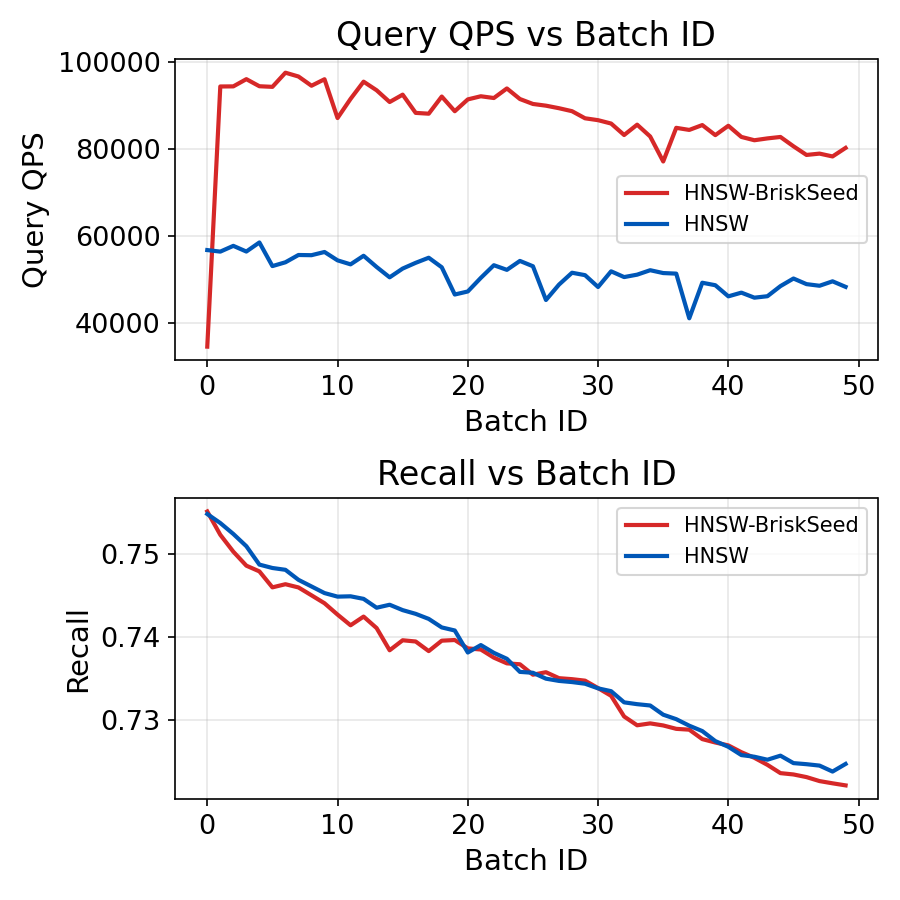
\includegraphics[width=0.31\textwidth]{figures/sift.png}
    }\hfill
    \subfloat[Msong]{
        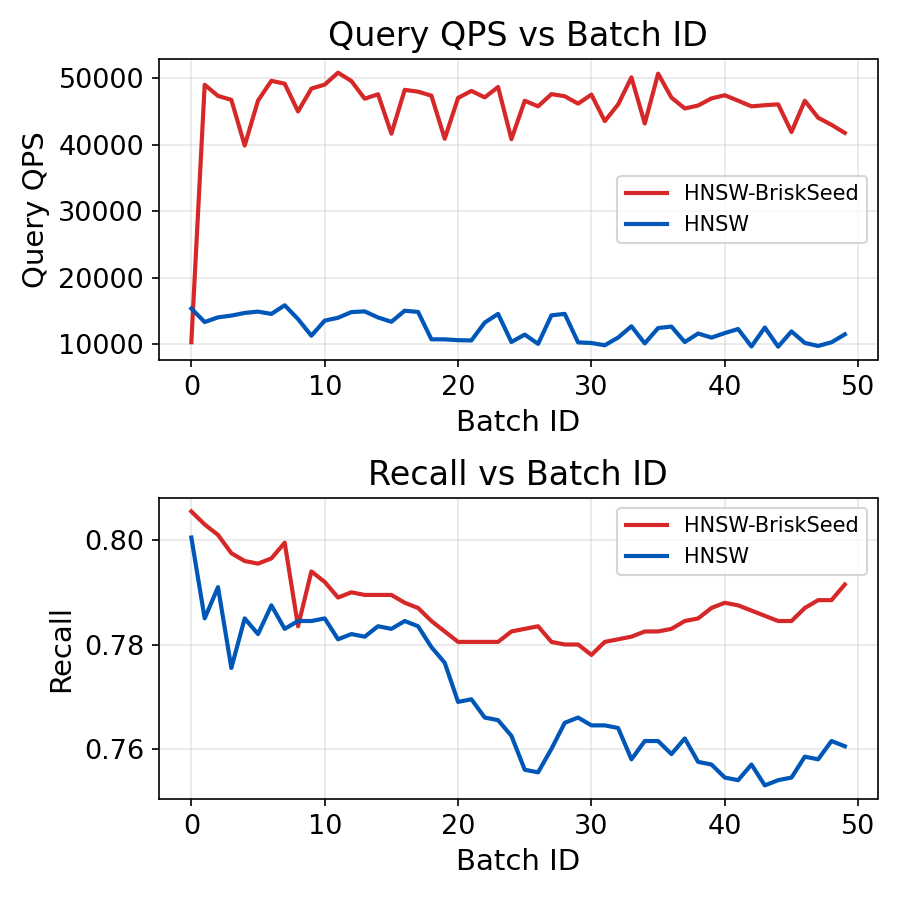
\includegraphics[width=0.31\textwidth]{figures/msong.png}
    }\hfill
    \subfloat[Glove]{
        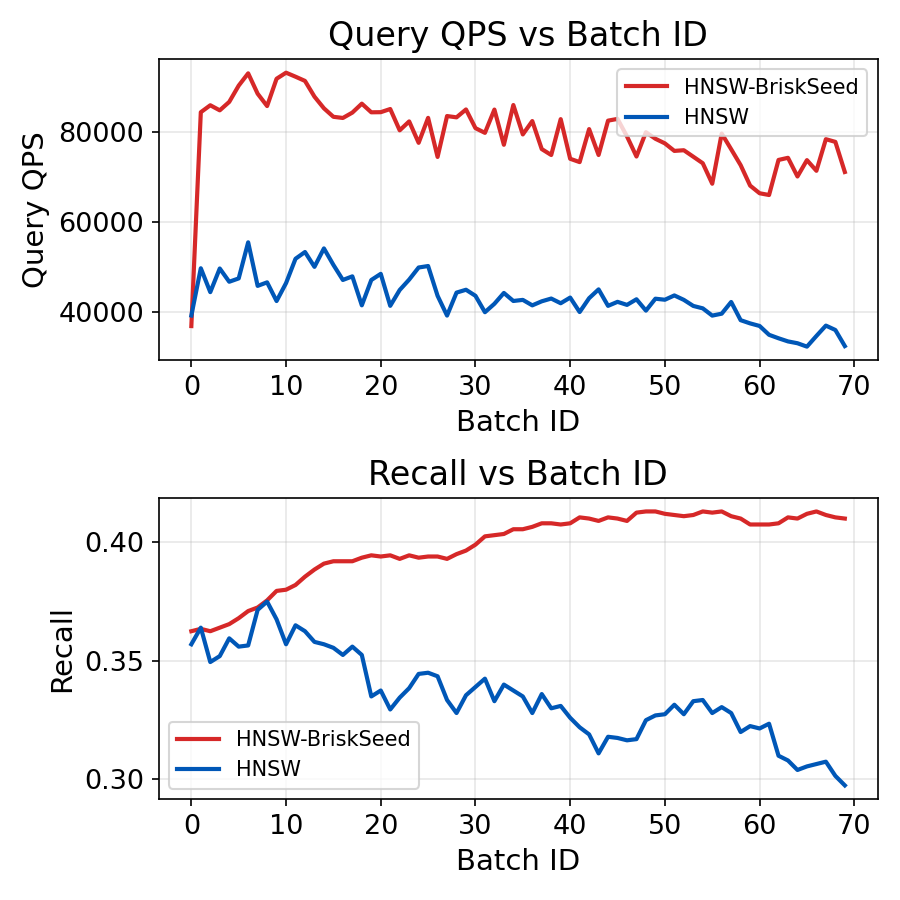
\includegraphics[width=0.31\textwidth]{figures/glove.png}
    }
    \caption{QPS and Recall comparison between the baseline and \system on three datasets.}
    \label{fig:qps-recall-three-datasets}
\end{figure*}

\subsection{Memory Usage}

\subsection{Ablation Study}

\subsection{Parameter Study}

\subsection{Scaling-up Study}
\section{Related Work}

\subsection{Most Directly Related: Dynamic and Graph-based ANNS}
Graph-based methods such as HNSW and its variants are widely adopted for high-recall and low-latency vector search.
Most designs, however, are optimized for static or slowly changing datasets, where index quality and auxiliary search artifacts are built offline.
Recent dynamic ANNS studies explore incremental index maintenance and update-aware operations.
In contrast, StreamSeed focuses on policy-level control of query hint reuse and provides a pluginized path to integrate with existing dynamic backends.

\subsection{Indirectly Related: System and Algorithm Acceleration}
Prior system works improve ANNS throughput via hardware-conscious layouts, vector quantization, and SIMD-friendly distance computation.
These approaches are complementary to StreamSeed: they optimize execution efficiency but do not directly address online staleness of reusable query guidance.
Algorithmic methods reduce unnecessary distance evaluations through pruning, lower-bound estimation, or partial-dimension strategies.
While effective in static contexts, they usually rely on assumptions that weaken under high-rate updates and distribution drift.

\subsection{Other: Positioning of This Work}
StreamSeed is orthogonal to both system-only and algorithm-only accelerations.
Its contribution is a unified online control loop (AQHC) that jointly manages hint construction, usage, and update,
bridging algorithmic reuse opportunities with systems-level deployability in streaming settings.

\section{Conclusion}
In this work, we study query acceleration for ANNS under dynamic updates. Existing acceleration methods face a fundamental tension: search hints constructed for static snapshots quickly become stale as updates arrive, while frequent global re-optimization incurs high maintenance overhead and can offset the intended throughput gains. To address this challenge, we propose \system, a lightweight dynamic acceleration plugin that turns static hinting into an online reuse--validate--refresh loop. \system maintains bounded reusable seed states and combines exact reuse on hot paths with semantic retrieval, bounded neighbor expansion, and fallback validation to preserve recall while improving end-to-end efficiency. We further present an analytical model for practical parameter instantiation under budget constraints. Extensive experiments show that \system consistently improves throughput, preserves competitive recall, and delivers robust performance under dynamic update workloads.



\bibliographystyle{IEEEtran}
\bibliography{reference}
\end{document}
